\documentclass[a4paper,12pt]{article} % добавить leqno в [] для нумерации слева

\usepackage{lab_preamble}

\begin{document}

\LabTitle {1.4.1} {Изучение экспериментальных погрешностей на примере физического маятника}

\textbf{Цель работы}:
\begin{enumerate}
\item На примере измерения периода свободных колебаний физического маятника познакомиться с систематическими и случайными погрешностями, прямыми и косвенными измерениями;
\item Проверить справедливость формулы для периода колебаний физического маятника и определить значение ускорения свободного падения;
\item Убедиться в справедливости теоремы Гюйгенса об обратимости точек опоры и центра качания маятника;
\item Оценить погрешность прямых и косвенных измерений и конечного результата.
\end{enumerate}

\textbf{Приборы}:
\begin{enumerate}
\item Металлический стержень с опорной призмой
\item Дополнительный груз
\item Закреплённая на стене консоль
\item Подставка с острой гранью для определения цента масс маятника
\item Прибор для измерения периода колебаний (секундомер) $ \sigma_T \sim 0,03 $
\item Счётчик колебаний (механический или электронный)
\item Линейки металлические различной длины
\item Штангенциркуль
\item Электронные весы
\item Математический маятник (небольшой груз, подвешенный на нитях)
\end{enumerate}

\section{Краткая Теория.}

Физическим маятником называют твёрдое тело, способное совершать колебания в вертикальной плоскости, будучи подвешено за одну из своих точек в поле тяжести. Основное отличие физического маятника от математического в том, что маятник не является точечным объектом,
а представляет собой совокупность жёстко связанных точечных масс. В данной работе в качестве такого маятника используется тонкий однородный металлический стержень, подвешиваемый в некоторой точке с помощью небольшой опорной призмы (см. рис. 1). Острое ребро
призмы, опирающееся на подставку, задаёт ось качания (или вращения) маятника.

Рассмотрим тело P и ось S.
Моментом инерции P отн. S называется $J = \sum_i {m_i \cdot r_i^2}$ (или $\int_{P} {r^2 \cdot dm}$ если масса P распределена равномерно), где $r_i$ - расстояние от $m_i$ до S.
Момент импульса тела: $L = J*\omega$, где $\omega$ - угловая скорость вращения тела отн. оси S.
Момент импульса: \[M = \frac{dL}{dt} (1) = J \cdot \frac{d\omega}{dt} (2)\]

\begin{figure} [h]
\center
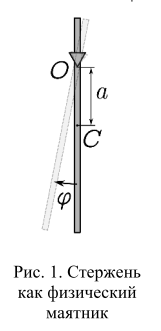
\includegraphics[scale=0.8]{./141/pic1.png}
\end{figure}

Справедлива следующая формула для тонкого стержня массы m и длины l, вращающегося вокруг оси, проходящей через центр масс: $J_c = \frac{m \cdot l^2}{12}$.
А для такого же стержня, подвешенного на расстоянии a от центра масс, момент инерции может быть вычислен по формуле Гюйгенса-Штейнера: \[J = \frac{m \cdot l^2}{12} + m \cdot a^2 \ (3)\]
В частности, если подвесить стержень за один из концов: $a = \frac{l}{2} \implies J = \frac{m \cdot l^2}{3}$

Вернёмся к рассмотрению колебаний физического маятника — стержня, подвешенного в поле тяжести (Рис. 1). Маятник подвешен в точке O на расстоянии a до центра масс C. При отклонении стержня от вертикального положения равновесия на угол $\varphi$ возникает момент силы тяжести, стремящийся вернуть стержень в исходное положение. Плечо этой
силы, приложенной к точке C, относительно оси подвеса O равно $a \cdot \sin{\varphi}$,
поэтому при небольших углах отклонения $\varphi \ll 1$ возвращающий момент
равен: \[M\ =\ -m \cdot g \cdot a \cdot \sin{\varphi} \approx -m \cdot g \cdot a \cdot \varphi \ (4)\]
Отсюда можно сделать вывод о том, что такие колебания будут гармоническими при малых амплитудах.
Для гармонических колебаний: $T\ =\ 2\pi \cdot \sqrt{\frac{m}{k}}$, T - период колебаний.
Аналогично для физического маятника: $m\ =\ J$, k - отношение момента силы к амплитуде, $k\ =\ mga$. Отсюда \[T\ =\ 2\pi \cdot \sqrt{\frac{J}{mga}} \ (5)\]
Для стержня: \[T\ =\ 2\pi \cdot \sqrt{\frac{\frac{l^2}{12} + a^2}{g \cdot a}} \ (6)\]
Для математического маятника: \[T\ =\ 2\pi \cdot \sqrt{\frac{l}{g}} \ (7)\]

По опр. приведенная длина: $l_{\text{пр}} = a + \frac{l^2}{12a}$. Смысл данной величины в том, что физический маятник длины l и подвешенный на расстоянии a имеет тот же период малых колебаний, что и математический маятник длины $l_{\text{пр}}$.

\begin{figure} [h]
\center
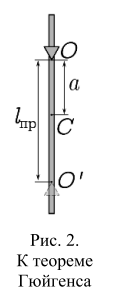
\includegraphics[scale=0.8]{./141/pic2.png}
\end{figure}

\center{Гармонические колебания}
\[(1),(4) \implies J \ddot{\varphi} + mga \varphi \ = \ 0\ (9)\]
\[\varphi(t) = A \sin{(\Omega t + \alpha)}\ (10)\], где $\Omega = \frac{2\pi}{T} = \sqrt{\frac{mga}{J}}$ - угловая частота колебаний, A - амплитуда, $\alpha$ - начальная фаза колебаний.

\center{Затухание колебаний}
Если присутствует сила трения, затухания считаются затухающими. Для затухающих колебаний формула (10) справедлива, но амплитуда является убывающей ф-ией от времени: A = A(t).
Декремент затухания: $\gamma = \frac{| \Delta A |}{A}$
\[\gamma = const \implies \gamma = -\frac{dA}{A} \implies A(t) = A_0 \cdot e^{-\gamma t}\], где $A_0 = A(0)$. \newline
$\tau = \frac{1}{\gamma}$ - время, за которое амплитуда падает в e раз.
Колебания можно считать малым, если $\tau >> T$.
Добротность колебательной системы: $Q = \pi \frac{\tau}{T}$

\center{Эксперементальная установка}
Тонкий стальной стержень длиной $l \sim 1$ м и массой $m \sim 1$ кг (точные параметры определяются непосредственными измерениями) подвешивается на прикреплённой стене консоли с помощью небольшой призмы. Диаметр стержня много меньше его длины $d \sim 12$ мм << l . Небольшая призма
крепится на стержне винтом и острым основанием опирается на поверхность закреплённой на стене консоли. Острие ребра призмы образует ось качания маятника.
Возможны две схемы реализации установок:

\textbf{Установка A.} Призму можно перемещать вдоль стержня, изменяя длину a — расстояние от центра масс до точки подвеса. Период колебаний измеряется непосредственно с помощью секундомера.

\textbf{Установка B.} Подвесная призма остаётся неподвижной (a = const), а на стержень маятника насаживается дополнительное тело небольшого размера («чечевица» или цилиндр), положение которого можно изменять, изменяя таким образом момент инерции маятника. Период колебаний маятника в этой схеме измеряется электронным счетчиком импульсов, расположенном у нижнего конца стержня. Дополнительные сведения об установке типа Б приведены ниже (см. стр. 8).

Измеряя зависимости периода малых колебаний от положения стержня или дополнительного тела на нём, можно экспериментально проверить формулу (5) (или её частный случай (6)) и вычислить значение ускорения свободного падения g. Формулу (6) можно проверить, откладывая по осям
величины $u = T^2$ a и $m = a$ 2 . В этих координатах график u(m) должен
иметь вид прямой линии, угловой коэффициент которой пропорционален g, а вертикальное смещение — моменту инерции стержня относительно центра масс.

\center{Измерение периода колебаний}
Дабы избежать слишком большой ошибки измерения времени ($\sigma_t = 0,1-0,3 c$), нужно измерить время несколько раз ({$t_1, t_2, ..., t_N$}) и найти случайную погрешность по формуле:
\[\sigma^{\text{случ}}_t = \sqrt{\frac{\sum{(t_i - <t>)^2}}{N-1}}\]
\[\sigma^{\text{полн}}_t = \sqrt{\sigma^{\text{сист}^2}_t + \sigma^{\text{случ}^2}_t}\]

\center{Особенности маятника с перемещаемым грузом (установка B)}
Масса грузика: $m_g = 300 - 400$ гр, диаметр: $d_g \sim 6$см

\begin{figure} [h]
\center
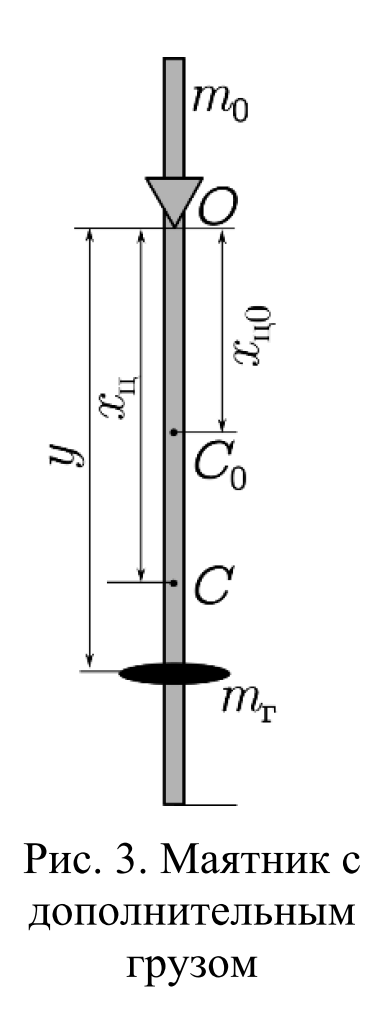
\includegraphics[scale = 0.3]{./141/pic3.png}
\end{figure}

\[J = J_0 + m_{\text{г}} \cdot y^2\]
где $J_0$ — момент инерции маятника без груза, определяемый по формуле (3).

\[x_{2} = \frac{m_0 \cdot x_{1} + m_g \cdot y}{M}\]

\[y = \frac{M \cdot x_{2} - m_0 \cdot x_{1}}{m_g} \ (12)\]

\[T\ =\ 2\pi \cdot \sqrt{\frac{J_0 + m_g \cdot y^2}{g\ M\ x_2}} \ (13)\]

\center{Учёт влияния подвесной призмы}

Формула (6) получена в предположении, что подвес маятника является материальной точкой. На самом же деле маятник подвешивается с помощью треугольной призмы конечного размера, поэтому использование (6) может привести к систематической погрешности результата. Для более точных расчётов следовало бы воспользоваться общей формулой периода колебаний физического маятника (5), принимая во внимание наличие двух тел — стержня и призмы:

\[T = 2\pi \sqrt{\frac{J_{\text{пр}} + J_{\text{ст}}}{m_{\text{пр}}\ g\ a_{\text{пр}} - m_{\text{ст}}\ g\ a_{\text{ст}}}}\],
где $J_{\text{пр}}$, $m_{\text{пр}}$ и $a_{\text{пр}}$ — соответственно момент инерции, масса и расстояние
до центра масс призмы (знак «минус» в знаменателе учитывает, что призма находится выше оси подвеса).

$m_{\text{пр}} \sim 70gr,\ a_{\text{пр}} \sim 1.5cm \implies J_{\text{пр}} = m_{\text{пр}}\cdot a_{\text{пр}}^2 \sim 10^{-5} kg\ m^2$ $a_{\text{ст}} = 10cm \implies J_{\text{ст}} \sim 10^{-2}\ kg\ m^2$
$\implies \xi_{J_{\text{ст}}} < 0.1\%$

\[\frac{M_{\text{пр}}}{M_{\text{ст}}} = \frac{m_{\text{пр}}\ g\ a_{\text{пр}}}{m_{\text{ст}}\ g\ a_{\text{ст}}} \sim 1\%\]

\section{Выполнение работы.}
\begin{enumerate}

\item Ознакомимся с используемыми в работе измерительными приборами: линейкой, штангенциркулем, секундомером.
Определим максимальную систематическую погрешность каждого из них (абсолютное и относительное значение) (смотрите таблицу 1).
Оценим, с какой относительной погрешностью имеет смысл измерять период колебаний маятника. Погрешность итогового результата (косвенно вычисленной величины) не может оказаться больше погрешности самого неточного измерения.
В нашем случе относительная погрешность самого неточного измерения равна примерно $1\%$.
Если период маятника примерно равен 1 секунде в нашем случае относительная погрешность измерения одного периода равняется $\varepsilon_T = \frac{\sigma_T}{T} \sim \frac{0.03}{1} = 0.03 = 3\%$. Тогда будет достаточно измерения 3 колебаний. Для большей точности будем измерять период 20 колебаний.

\item Измерим длину стержня $L_{\text{ст}}$ . Взвесим стержень, призму и дополнительный
груз ($M_{\text{ст}} = 868 \text{г}, M_{\text{пр}} = 80 \text{г}, M_{\text{гр}} = 291 \text{г}$) (для установки Б) на электронных весах. Оценим погрешности
измерений (абсолютные и относительные значения) (см. т. 1).

\begin{figure} [h]
	\center
	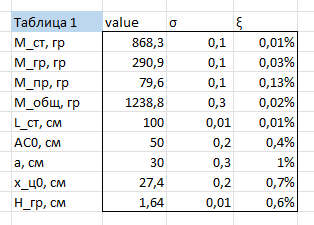
\includegraphics[scale = 0.8]{./141/таблица 1.png}
\end{figure}

\item Снимем со стержня призму и с помощью подставки определим положение центра масс пустого стержня.
$AC0 = (50 \pm 0,2)\text{см}$

\item Установим призму на некотором расстоянии от центра стержня, измерим точное положение от острия призмы до центра масс
стержня - $a = P_rC_0$.
Измерим положение центра масс конструкции $x_{\text{ц0}} = P_rC_1$, сбалансировав маятник с призмой на острие вспомогательной подставки. Оценим погрешности измерения расстояний a и $x_{\text{ц0}}$.
$\sigma_a = 0.3\text{мм};\ \sigma_{x_{\text{ц0}}} = 0.2\text{мм}$
$a = (30.0 \pm 0.3)\text{см};\ x_{\text{ц0}} = (27.4 \pm 0.2)\text{см}.$
$\varepsilon_a = 1\%;\ \varepsilon_{x_{\text{ц0}}} = 0.7\%$

\item Проведем первый предварительный опыт по измерению периода колебаний (на установке Б опыт проведите без дополнительного груза).
\begin{enumerate}
	\item[а) ] Установим маятник на консоли и отклоним маятник на малый угол (не более $ 5 \degree $). Убедимся, что он качается без помех, призма не проскальзывает, и колебания затухают слабо.
	\item[б) ] Измерим время n = 20 полных колебаний маятника.
	\item[в) ] Вычислим период колебаний $T = \frac{d}{n}$ и по формуле (6) (или (14)) рассчитайте предварительное значение g. Убедитесь, что оно отличается от табличного не более, чем на $10\%$.
\end{enumerate}

$T_{\text{ср}} \sim 1.5 \text{с}$
По формуле (6): $g = \frac{4\pi^2}{T^2} \cdot \frac{\frac{l^2}{12} + a^2}{a} \sim 9.52 \frac{\text{м}}{\text{с}^2} \implies \varepsilon_g \sim 2.8\%$
По формуле (14): $g = \frac{4\pi^2}{T^2} \cdot \frac{\frac{l^2}{12} + a^2}{x_{\text{ц}}(1 + \frac{m_{\text{пр}}}{m_{\text{ст}}})} \sim 9.55 \frac{\text{м}}{\text{с}^2} \implies \varepsilon_g \sim 2.5\%$

\item Проведем серию измерений для экспериментального определения случайной погрешности измерения периода.
\begin{enumerate}

	\item Несколько раз повторим измерение периода фиксированного числа колебаний (например, при n = 20). Результаты занесем в таблицу. Если результаты 3–4 измерений полностью совпадают, опыт можно остановить. Если результаты
		различаются, следует провести 8–10 измерений.
		В нашем случае результаты немного разнились, поэтому мы провели 10 измерений периода (см. таблицу 2).

		\begin{figure} [h]
			\center
			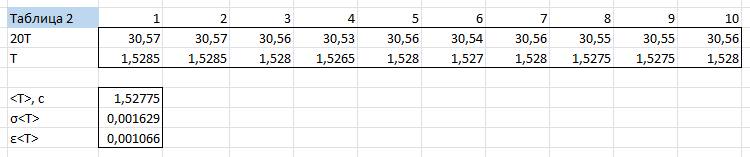
\includegraphics[scale = 0.8]{./141/таблица 2.png}
		\end{figure}

	\item Вычислим среднее значение полученных результатов $\overline{t} \sim 1.53\text{с}$, а также определим случайную погрешность измерения времени как среднеквадратичное отклонение полученных результатов:
		$\sigma_t^{\text{случ}} = \sqrt{\frac{1}{N-1} \cdot \sum_{i = 1}^{N}{(t-\overline{t})^2}} \sim 6*10^{-4}\text{с}$, где N - число измерений, в нашем случае N = 10.

	\item Определим приборную (систематическую) погрешность используемого прибора $\sigma_t^{\text{сист}}$ и вычислим полную погрешность $\sigma_t^{\text{полн}}$ измерения времени.
		$\sigma_t^{\text{сист}} = 0.03\text{с} \implies \sigma_t^{\text{полн}} = \sqrt{\sigma_t^{\text{случ}^2} + \sigma_t^{\text{сист}^2}} \sim \sigma_t^{\text{сист}} = 0.03\text{с}$

\end{enumerate}

\item Используя погрешность $\sigma_t$ измерения времени из предыдущего пункта, оцените число колебаний n, по которому следует измерять период, чтобы относительная погрешность измерений периода соответствовала точности измерений $\varepsilon_{max}$, оценённой в п. 1.
Так как мы измеряли период электронным счетчиком, полная погрешность примерно равна приборной, следовательно, размышления в п. 1 справедливы.

\item Закрепим груз на стержне в произвольном месте. Рассчитаем положение центра масс стержня, призмы и груза:
\[x_{\text{ц}} = P_rC_2 = \frac{(M_{\text{ст}} + M_{\text{пр}}) x_{\text{ц0}} + M_{\text{гр}} \cdot y}{M_{\text{ст}} + M_{\text{пр}} + M_{\text{гр}}}\], где y - расстояние от т. подвеса до груза.

\item Разместим груз на маятнике и измерим положение y груза относительно точки подвеса и положение центра масс всей системы $x_{\text{ц}}$.

\item Проведем измерение периода колебаний маятника по n полным колебаниям, где значение n выбрано в п. 7. Повторим измерения периода для 8 - 15 положений груза y (при этом распределим положения груза равномерно по всему стержню). Для каждого измерения найдем $x_{\text{ц}}$ и g (см. т. 3).

\begin{figure} [h]
	\center
	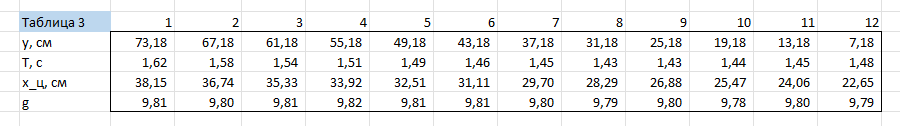
\includegraphics[scale = 0.7]{./141/таблица 3.png}
\end{figure}

\item Не выполняли.

\item Оценим затухание маятника, для этого измерим время, за которое амплитуда колебаний уменьшится вдвое - ($\tau \sim 8\ \text{мин}\ 30\ \text{сек}$, и $\tau_{\text{зат}} = \frac{\tau}{\ln{2}} \sim 735\ \text{сек}$, тогда декремент затухания $\gamma = \frac{1}{\tau_{\text{зат}}} \sim 1.4 \cdot 10^{-4}\ \text{сек}^{-1}$, а добротность $Q = \pi \frac{\tau_{\text{зат}}}{T} \sim 1500$). Погрешность добротности посчитать невозможно.

\section{Обработка результатов измерений.}

\item Усредним значения g из таблицы 3 и оценим погрешность.
$g \sim 9,8 \frac{\text{м}}{\text{с}^2}\ (9,55),\ \sigma_g = 1,12 \frac{\text{м}}{\text{с}^2}\ (1,15),\ \varepsilon_g = 1,2\%\ (1,6)$.

\item Построим график зависимости T от y.

\begin{figure} [h]
	\center
	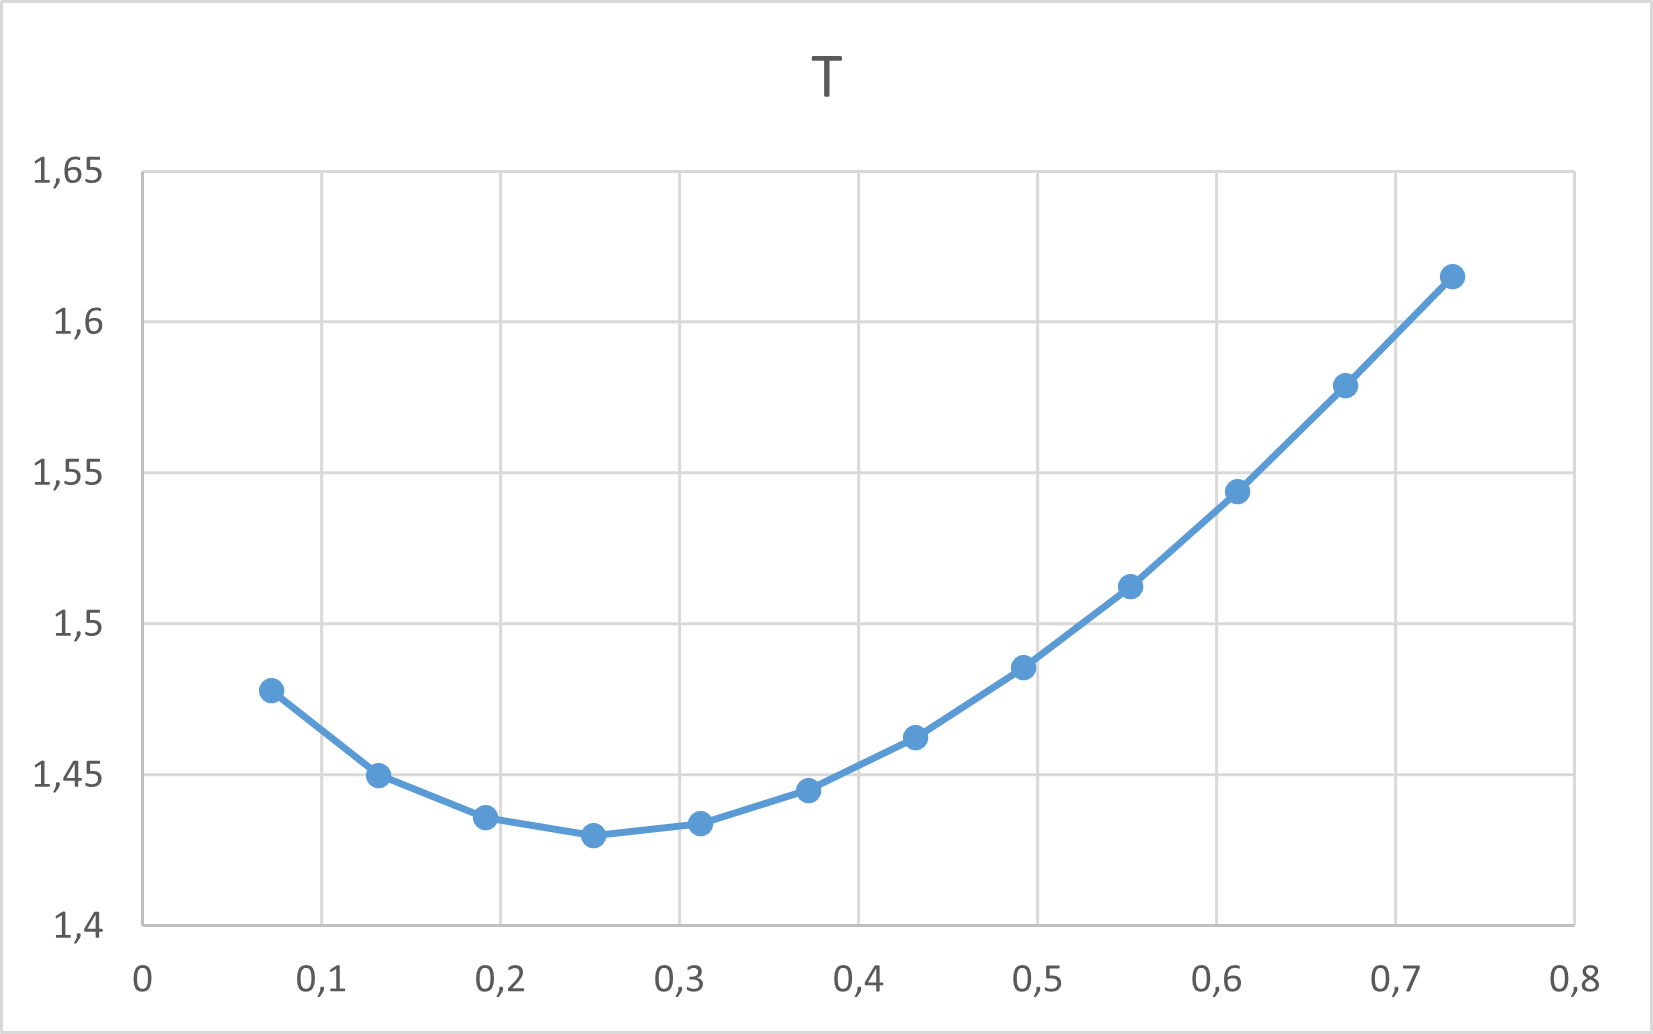
\includegraphics[scale = 0.8]{./141/T(y).png}
\end{figure}

Этот график имеет вид $T = a\sqrt{\frac{b+c \cdot y^2}{d+e \cdot y}} = \sqrt{\frac{J_0 + m_{\text{г}} \cdot y^2}{g (x_{\text{ц0}} m_{\text{ст}} + y \cdot m_{\text{г}})}}$,
$b = J_0,\ c = m_{\text{г}},\ d = x_{\text{ц0}} m_{\text{ст}},\ e = m_{\text{г}}$
Минимум ф-ии T(y) можно определить, решая ур-ие
$\frac{d}{dy} T = 0 \implies y_{min} = \sqrt{\frac{d^2}{e^2} + \frac{b}{c}} - \frac{d}{e} =
	\frac{x_\text{ц0} m_\text{ст}}{m_\text{г}} \cdot (\sqrt{\frac{J_0 m_\text{г}}{x_\text{ц0}^2 m_\text{ст}^2} + 1} - 1) \sim 27\ \text{см}$.
По графику видно, что минимум достигается в точке $ y_{min} = 25 \text{см} $, в этом случае ошибка равна шагу, с которым мы перемещали груз, т.е. 6 см.
$ y_{min} = (25 \pm 6)\ \text{см} $.

\item Построим график зависимости $u(v)$, где $u = T^2 \cdot x_{\text{ц}}$ и $v = y^2$ (см. рисунок 4). График u(v) должен получиться линейным, так как, по формуле (13), $u = 4\pi^2 \frac{J_0}{gM} + 4\pi^2 \frac{m_{\text{г}}}{gM} = a + b \cdot v$, где $J_0$ - момент инерции маятника отн. подвеса.

\begin{figure} [h]
	\center
	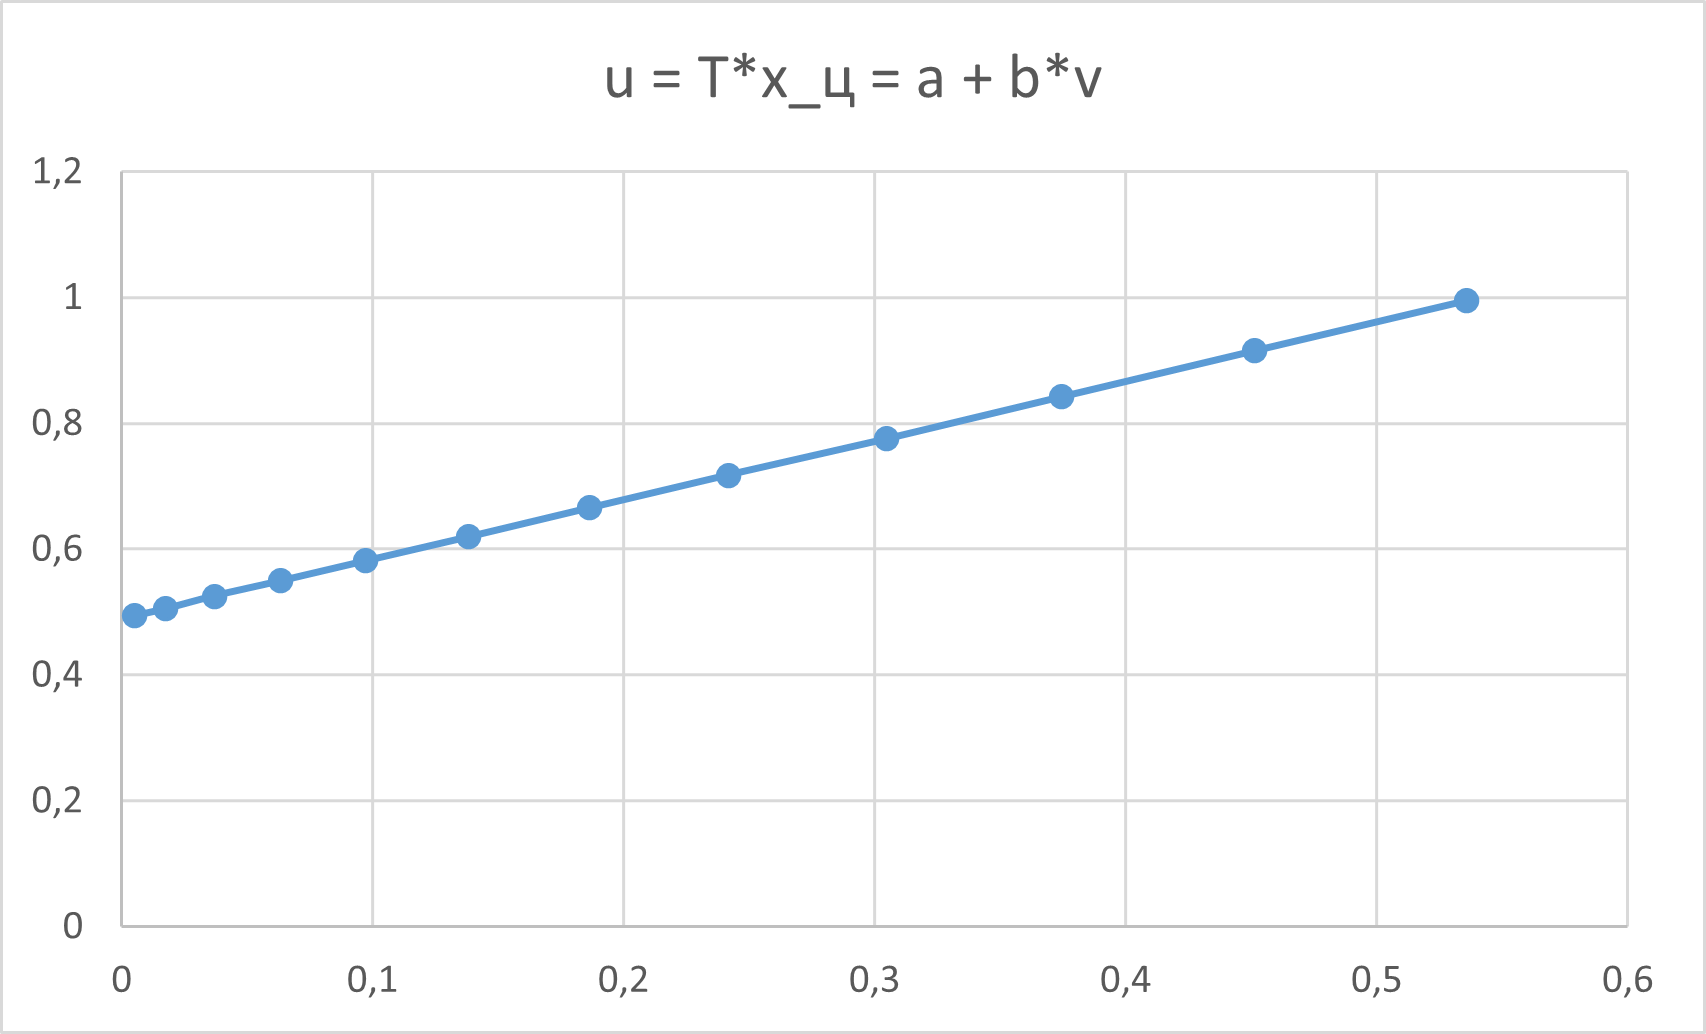
\includegraphics[scale = 0.8]{./141/u(v).png}
\end{figure}

\item Найдем коэффициент наклона (b) и пересечение с осью ординат (a) прямой u(v) (мы воспользовались мнк). В результате $a = 0,4849 \pm 0,0008,\ b = 1,000 \pm 0,005\ ;\ a \sim 0,5\ ,\ b \sim 1$. Из коэффициентов a и b можно найти g ($g = 4\pi^2 \frac{J_0}{a \cdot M} = 4\pi^2 \frac{m_{\text{г}}}{b \cdot M}$).
В результате $ g = 9,83 \frac{\text{м}}{\text{с}^2}\ (9,27)$

\item Найдем погрешность измерения g в п. 16.
$ \sigma_g = \sqrt{\varepsilon_{m_{\text{г}}}^2 + \varepsilon_{M}^2 + \varepsilon_{b}^2} \sim 0,05 \frac{\text{м}}{\text{с}^2}, \varepsilon_g = \frac{\sigma_g}{g} \sim 0,5\% $

\item Метод нахождения g лучше в 16 пункте, чем в 13, т.к. ошибка меньше.

\item В резуьтате мы получили ускорение свободного падения g двумя способами. На нашей планете g варьируется от 9,78 на экваторе, до 9,82 на полюсах. Мы получили, что $ g = (9,80 \pm 0,12) \frac{\text{м}}{\text{с}^2}\ и\ g = (9,83 \pm 0,05) \frac{\text{м}}{\text{с}^2}$. Наше значение отличается от истинного на 0,15\%.

\textbf{Вывод:} \newline
В результате выполнения работы, мы убедились в справедливости формул для периода колебаний физического маятника, в справедливости теоремы Гюйгенса об обратимости точек опоры и центра качания маятника, определили ускорение свободного падения двумя способами.

\end{enumerate}

\end{document}